\section{Paracaídas y Sistema de Recuperación}

El sistema de recuperación del cohete PDA STARS tiene como función primordial desacelerar el vehículo desde el apogeo ($304,22\text{ m}$) hasta la superficie con una velocidad terminal nominal de \textbf{8,00 m/s}, permitiendo que la estructura aterrice sin daño alguno y asegurando que la duración total del vuelo se sitúe estrictamente dentro de la ventana reglamentaria de \textbf{40 a 50 segundos} para motores de clase F.

\subsection{Dimensionamiento Aerodinámico del Paracaídas}
El paracaídas consiste en un domo hemisférico de \textbf{40 cm de diámetro} ($D_p = 0,40\text{ m}$) confeccionado en tela ripstop nylon ripstop de 40 g/m² con baja porosidad, provisto de \textbf{ocho líneas de suspensión} de cuerda de nylon trenzado de 40 cm de longitud ancladas uniformemente en la periferia.

El área de referencia proyectada es:
\begin{equation}
    S_p = \frac{\pi D_p^2}{4} = \frac{\pi (0,40)^2}{4} \approx 0,1257\text{ m}^2
\end{equation}
Para una masa total en descenso de $m = 437\text{ g}$ ($0,437\text{ kg}$, tras la expulsión de propelente), una densidad atmosférica local $\rho = 1,05\text{ kg/m}^3$ y un coeficiente de arrastre experimental del paracaídas hemisférico $C_d = 0,78$, la velocidad terminal de descenso en equilibrio cuasi-estático es:
\begin{equation}
    v_{\text{term}} = \sqrt{\frac{2 m g}{\rho S_p C_d}} = \sqrt{\frac{2 \cdot 0,437 \cdot 9,81}{1,05 \cdot 0,1257 \cdot 0,78}} \approx \mathbf{8,00\text{ m/s}}
\end{equation}
Este valor coincide con una precisión de dos decimales con la simulación numérica oficial de OpenRocket ($7,998\text{ m/s}$ en \texttt{simulacion\_stellaris.csv}), lo que arroja un tiempo de descenso en paracaídas de:
\begin{equation}
    t_{\text{descenso}} = \frac{304,22\text{ m}}{8,00\text{ m/s}} \approx 38,0\text{ s}
\end{equation}
Sumado al tiempo de ascenso hasta el apogeo ($8,90\text{ s}$), el tiempo total de vuelo resulta en:
\begin{equation}
    t_{\text{total}} = 8,90\text{ s} + 38,0\text{ s} \approx \mathbf{47,86\text{ segundos}}
\end{equation}
posicionando al cohete en el centro de la ventana oficial de 40 a 50 segundos.

\subsection{Cálculo de Deriva Radial por Viento Cruzado}
Considerando una capa de viento atmosférico lateral constante de $v_w = 3,5\text{ m/s}$ (condición máxima admisible en rampa según el manual de seguridad), la deriva horizontal teórica máxima $R$ es:
\begin{equation}
    R = v_w \cdot t_{\text{descenso}} = 3,5\text{ m/s} \cdot 38,0\text{ s} \approx 133\text{ metros}
\end{equation}
Este radio proporciona un margen de seguridad de más de 117 metros respecto al límite de exclusión obligatorio de \textbf{250 metros} fijado en la circular oficial de Zonas de Recuperación del CCCD 2026.

\subsection{Diagrama del Tren de Recuperación y Protección Térmica}
Para evitar la separación accidental de módulos durante el shock de apertura (estimado en $8\text{ -- }10\text{ G}$ dinámicos), todos los elementos estructurales se encuentran unidos mecánicamente en un tren continuo mediante un cordón tubular de Kevlar ignífugo de \textbf{3,6 metros} (12 pies) de longitud:
\begin{itemize}[leftmargin=1.5em]
    \item \textbf{Punto 1 (Extremo Superior):} Sujeción a la ojiva mediante cáncamo roscado M4.
    \item \textbf{Punto 2 (Cuerpo Intermedio):} Fijación al ojal estructural integrado en la base de la bahía de carga útil (ensayado a tracción de 250 N), asegurando que la carga útil permanezca solidaria al cohete en todo momento conforme a la Sección 5 de la Guía de Carga Útil.
    \item \textbf{Punto 3 (Arnés del Paracaídas):} Vínculo a las 8 líneas de suspensión mediante nudo de ocho por seno y eslabón rápido.
    \item \textbf{Punto 4 (Extremo Inferior):} Anclaje al anillo de centrado superior de la bahía motriz.
\end{itemize}

\begin{figure}[H]
\centering
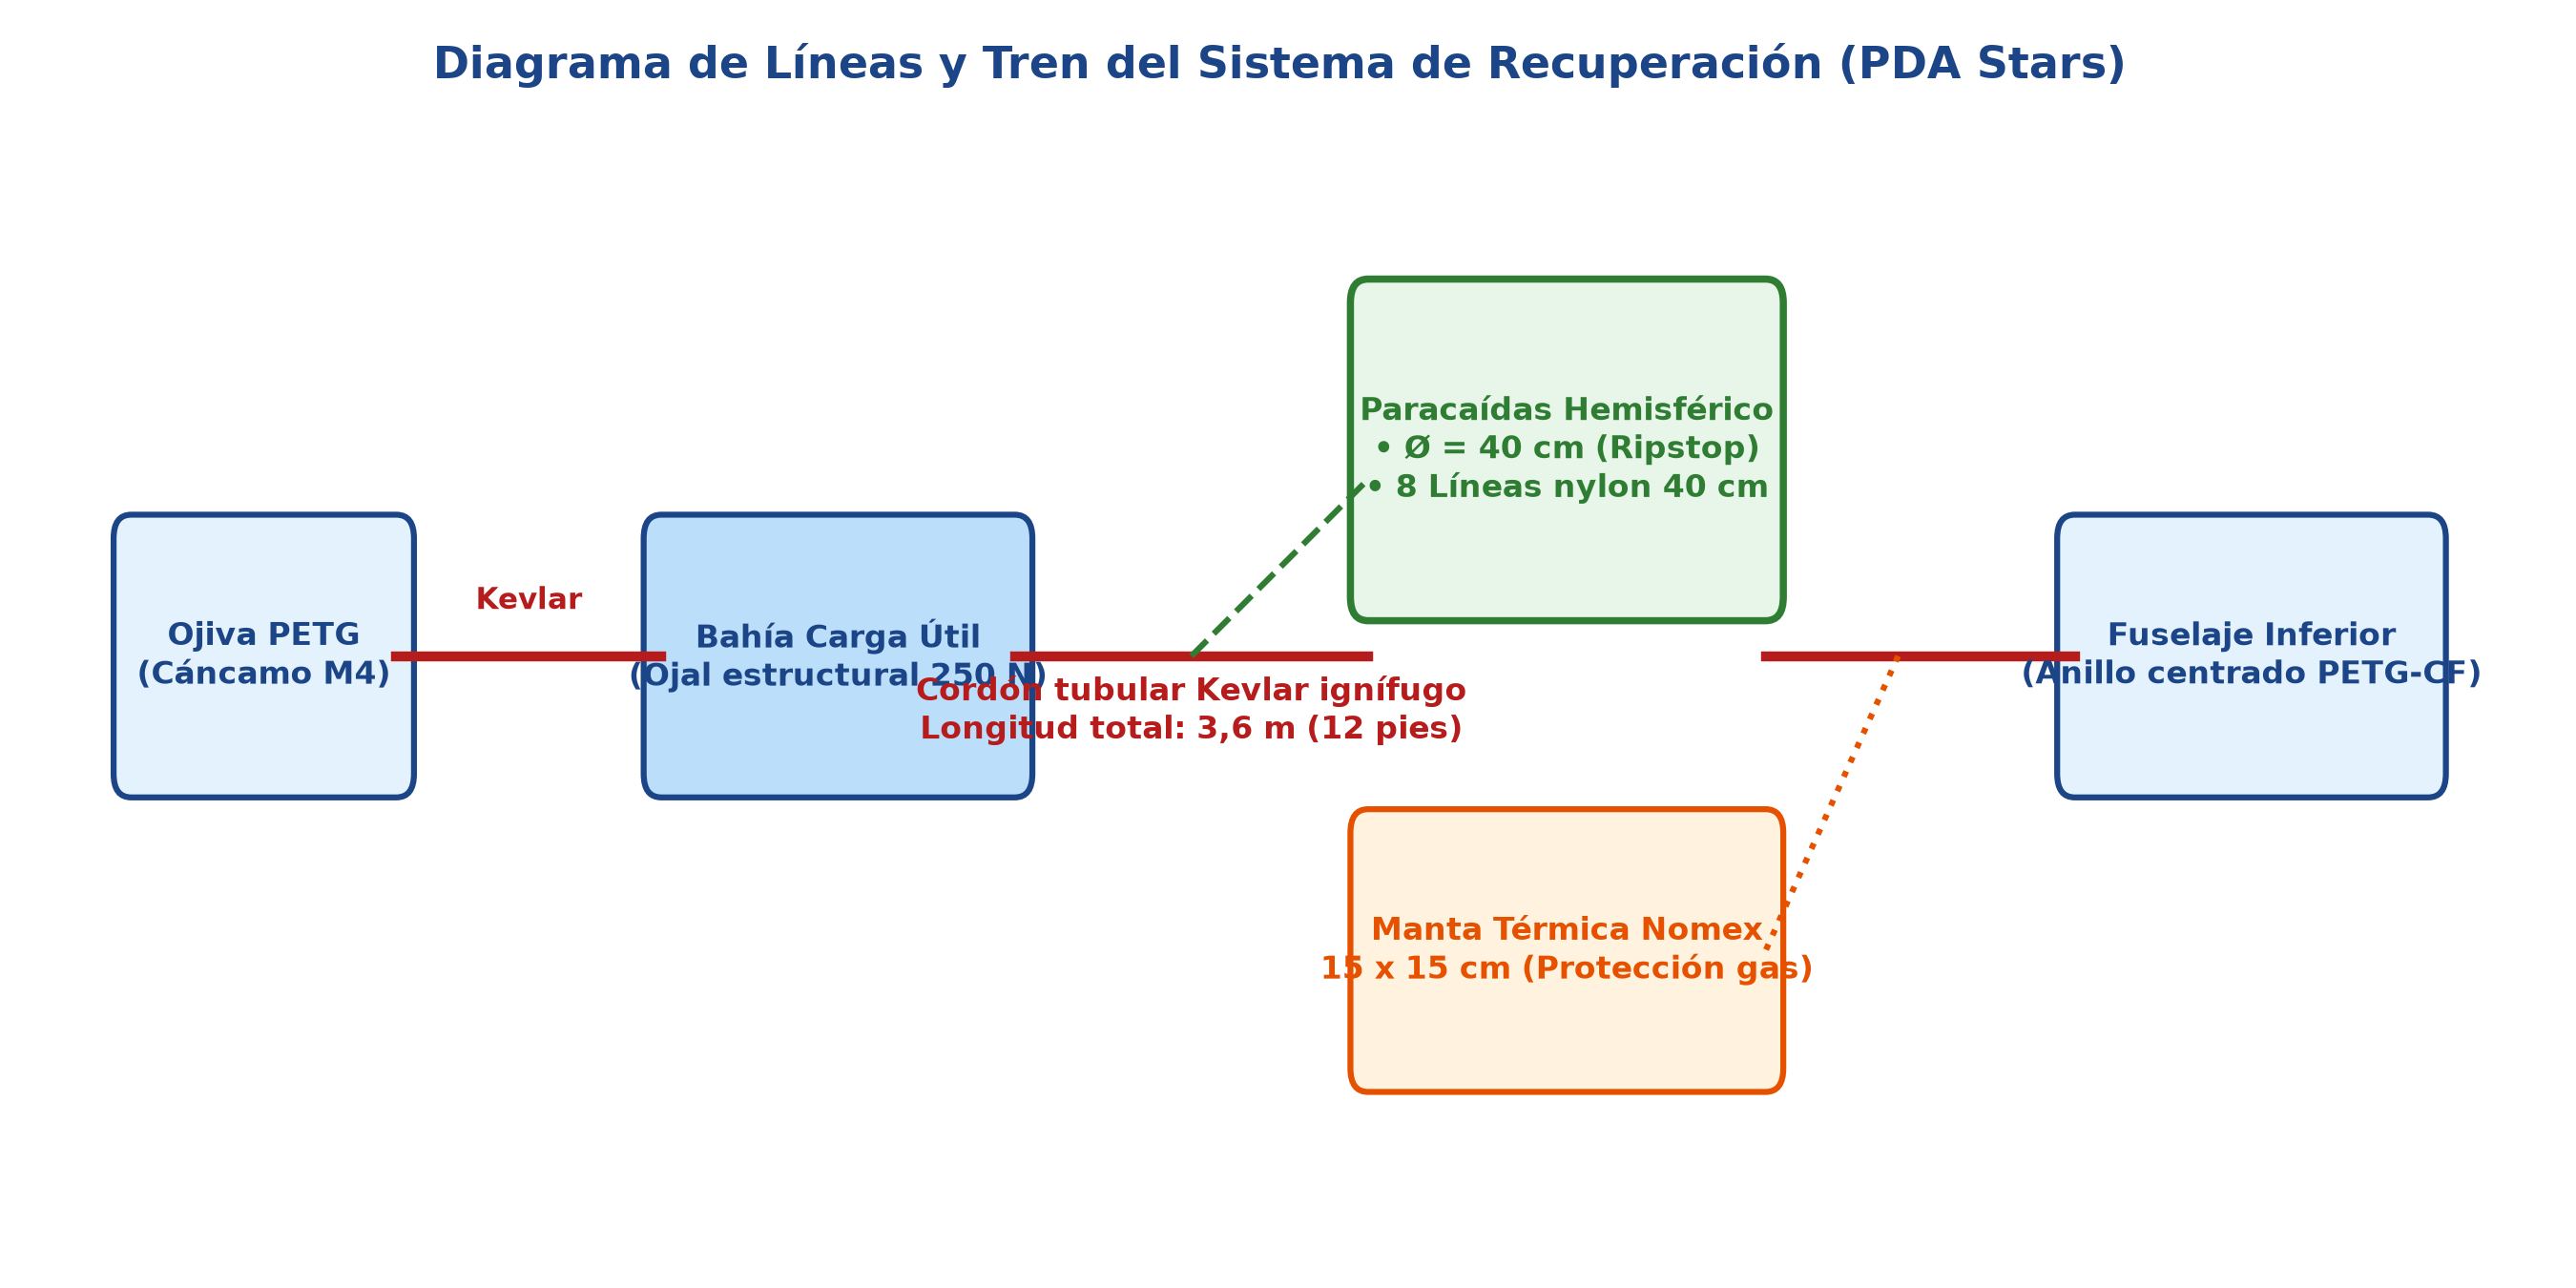
\includegraphics[width=0.92\linewidth]{fig_diagrama_lineas_recuperacion.png}
\caption{Diagrama esquemático de líneas y amarres del tren de recuperación de PDA STARS.}
\label{fig:diagrama_recuperacion}
\end{figure}

Para salvaguardar la tela de ripstop y las cuerdas de nylon del choque térmico generado por la carga de eyección de pólvora negra del motor F15-4 (retardo de 4 s), se intercala una \textbf{manta de protección térmica Nomex de 15x15 cm} (masa de 3,0 g) impregnada y doblada en acordeón sobre el tubo portamotor, sustituyendo por completo la necesidad de wadding desechable.
